%% APPLICATION NOTE OF BOON
%% Franck Delaplace 2024

\documentclass[numsec,webpdf,modern,large]{oup-authoring-template}

%\usepackage{showframe}
\usepackage{hyperref}
\usepackage[authoryear]{natbib}
\usepackage{graphicx}
\usepackage{xspace}
\usepackage{tikz}
\usepackage{tikz-network}
\usetikzlibrary{arrows,shapes}
\usepackage{tabu}

%% SET UP COLORS OF HYPERREF
\hypersetup{
	colorlinks=true,
	linkcolor=blue,      % Couleur des liens internes
	citecolor=blue,       % Couleur des citations
	urlcolor=blue    % Couleur des liens URL
}

\graphicspath{{figure/}} %% GRAPHIC PATH 

\newcommand{\boon}[0]{\textbf{BooN}\xspace}
%% STRUCTURE 
\newcommand{\tuple}[1]{\langle #1 \rangle}
\newcommand{\Bool}{{\mathbb B}}
\newcommand{\Nat}{{\mathbb N}}
\newcommand{\partset}[1]{\ensuremath{\textbf{2}^{#1}}} 
%% TRANSITION
\newcommand{\evo}[0]{\longrightarrow}
\newcommand{\xevo}[1]{\stackrel{#1}{\evo}}
\newcommand{\arc}{\ensuremath{\,\tikz[baseline=-0.5ex,scale=0.65,thin]{\draw[->,>=open triangle 45](0,0)to[bend left=0] (1,0);}\,}}
\newcommand{\shortarc}{\ensuremath{\,\tikz[baseline=-0.5ex,scale=0.45,thin]{\draw[->,>=open triangle 45](0,0)to[bend left=0] (1,0);}\,}}

%% ABBREVIATION
\newcommand{\abbrev}[1]{#1, \relax}
\newcommand{\ie}[0]{\abbrev{\textit{i.e.}}}
\newcommand{\eg}[0]{\abbrev{\textit{e.g.}}}
\newcommand{\cf}[0]{\abbrev{\textit{cf.}}}
\newcommand{\aka}[0]{\abbrev{\textit{a.k.a}}}

%% MATH
\newcommand{\eqdef}{\overset{\text{def}}{=\mathrel{\mkern-3mu}=}}
\newcommand{\Fix}[1]{\textsc{stbl}_{#1}}

\newcolumntype{C}{>{\centering\arraybackslash}X}
\renewcommand\arraystretch{1.2}

\begin{document}	
	\journaltitle{Bioinformatics}
	\DOI{DOI HERE}
	\copyrightyear{2024}
	\pubyear{XXX}
	\access{Advance Access Publication Date: Day Month Year}
	\appnotes{Paper}
	
	\firstpage{1}
	
	%\subtitle{Subject Section}
	
	\title[BooN]{BooN: Boolean Network Analysis Software}
	
	\author[1,$\ast$]{Franck Delaplace}
	%% \author[2]{Second Author}
	%%
	
	\authormark{Author Delaplace}
	
	\address[1]{\orgdiv{IBISC}, \orgname{Paris-Saclay University, Evry}, \orgaddress{ \country{France}}}
	%% \address[2]{\orgdiv{Department}, \orgname{Organization}, \orgaddress{\street{Street}, \postcode{Postcode}, \state{State}, \country{Country}}}

	\corresp[$\ast$]{Corresponding author. \href{email:franck.delaplace@univ-evry.fr}{franck.delaplace@univ-evry.fr}}
	
	\received{Date}{0}{Year}
	\revised{Date}{0}{Year}
	\accepted{Date}{0}{Year}
	
	
	\abstract{In this paper, we present an open source software, called \boon, which has been developed for the purpose of Boolean network analysis in Python. The release includes two main packages: one comprising a set of methods applied to the Boolean network object and the other for the graphical interface.  
	The software encompasses all the requisite features for Boolean network analysis, including graphical network design, interaction graph drawing, model of dynamics, symbolic computation of stable states, and controllability analysis.
	\section*{Availability and Implementation}
	 \boon  is freely available on \href{https://github.com/Franck-Delaplace/BooN}{GitHub} at \url{https://github.com/Franck-Delaplace/BooN}.
	 }.
	
	
	\keywords{Boolean Network, Controllability, Software}
	
	\maketitle
	\section{Introduction}
	\label{sec:introduction}

	Boolean Network Analysis applied to biological systems studies was pioneered by Stuart Kaufman\citep{kauffman1969,glass1973} and Ren\'e Thomas\citep{thomas1973} in 70s.
	 The objective was to develop a formal modeling framework for studying the dynamics of genetic networks, considering the available data for their analysis.
	 
	 Currently, this modeling framework is  regarded as the gold standard for studying biological systems, as evidenced by the substantial number of publications on biological network and system modeling (Figure~\ref{fig:publi}). Notably, these publications have significantly surpassed other modeling approaches in terms of prevalence.
	
	 One of the most significant challenges for this modeling framework concerns the development of software platforms facilitating their use by a large number of users with a diverse range of skill sets.
	 Such platforms should offer a comprehensive range of functionality and a user-friendly graphical interface.
	 	\begin{figure}[h!]
	 	\centering
	 	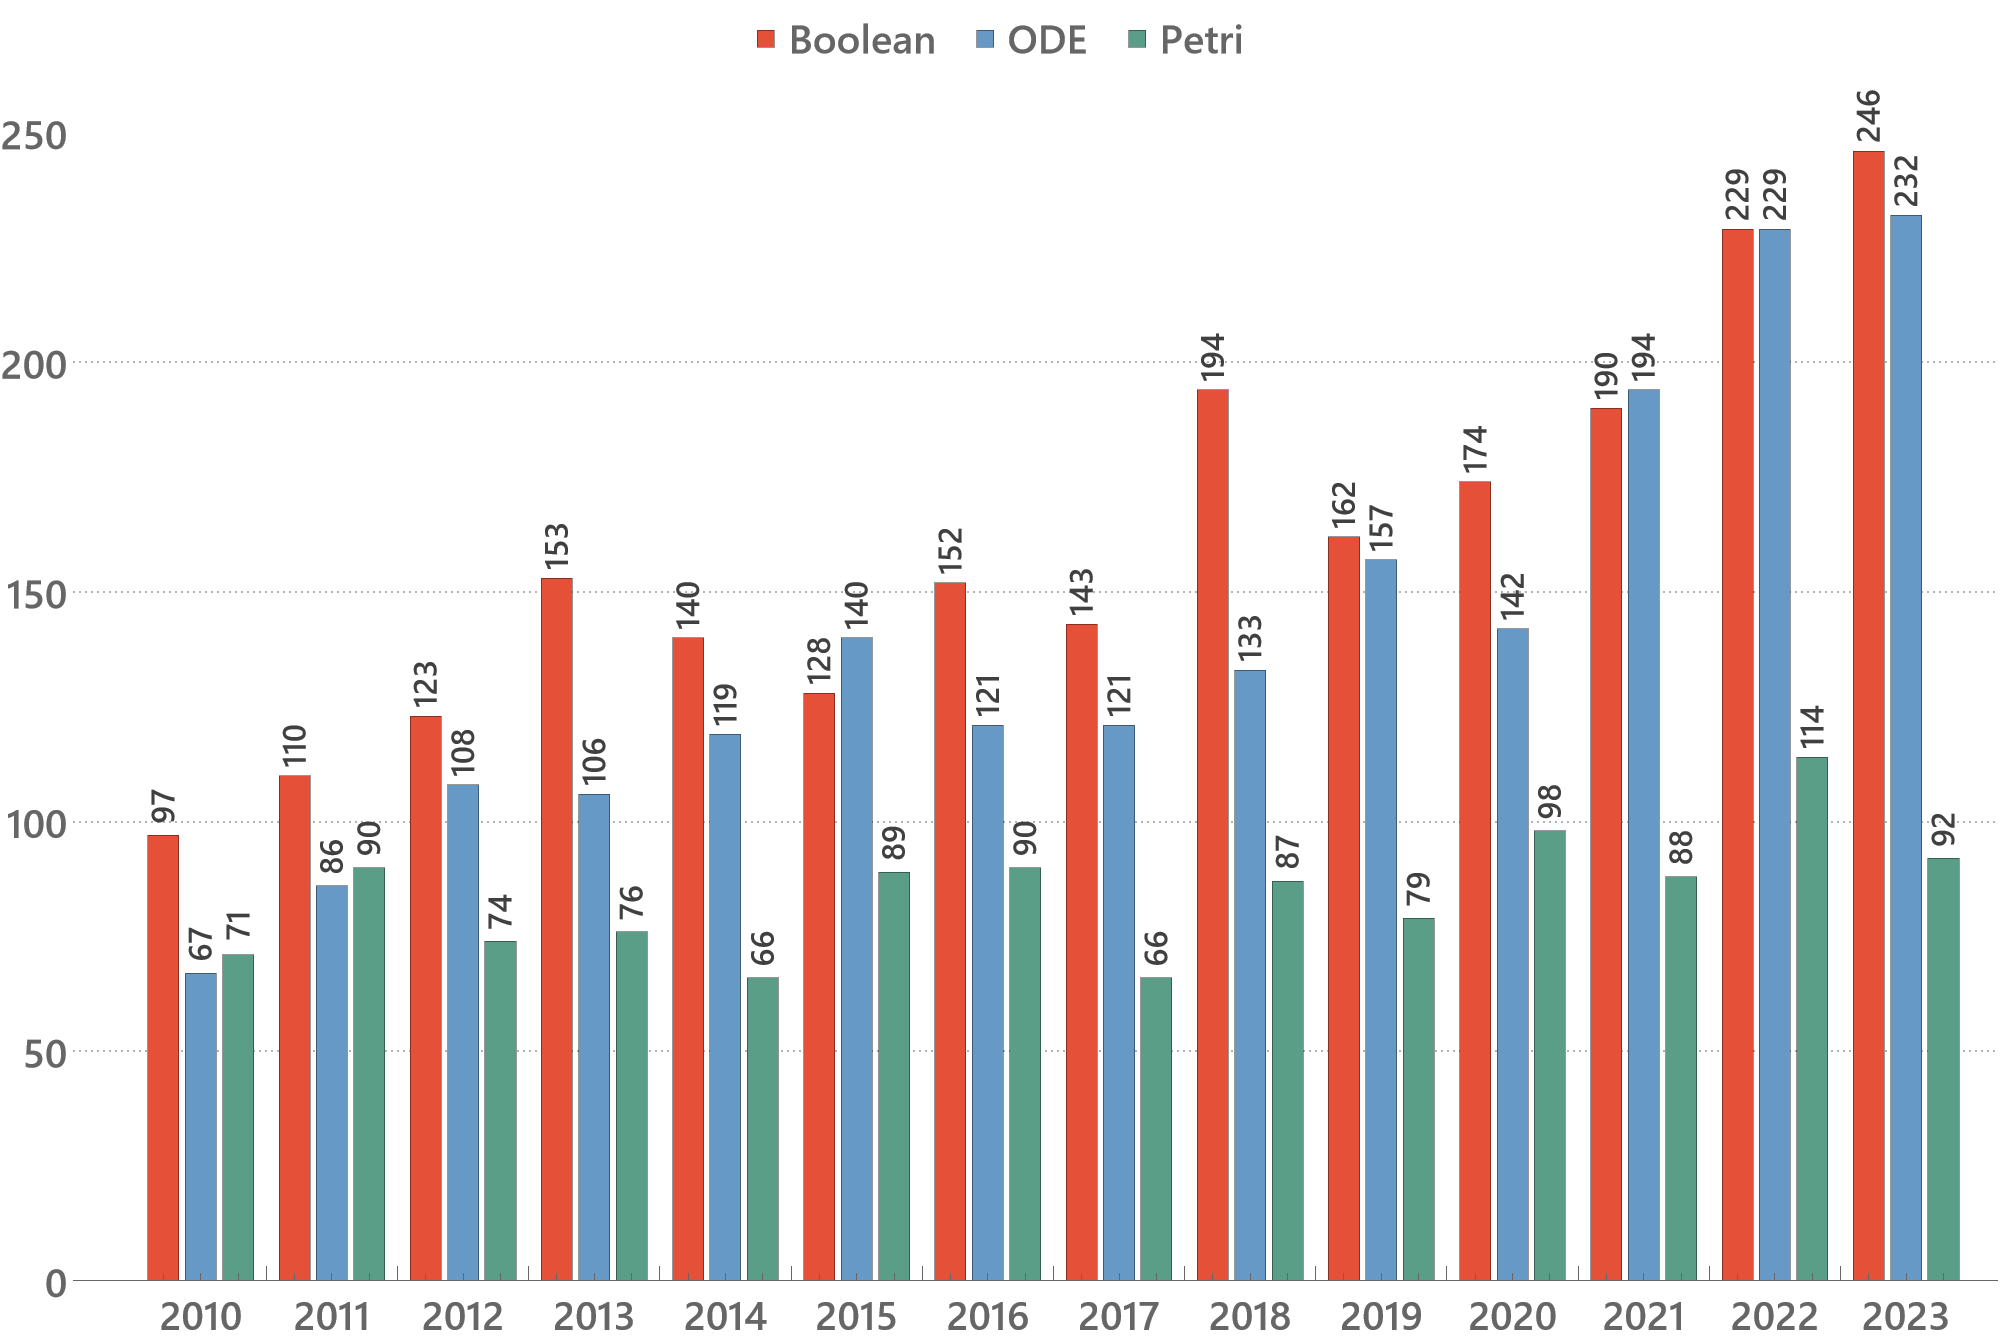
\includegraphics[width=0.45\textwidth]{pubmedmodelshort}
	 	
	 	%		\medskip
	 	%		\begin{tablenotes}%
	 		%			\item	$3$ queries were performed on \textsc{pubmed} to count the number of publications concerning Boolean, ordinary differential equation, and Petri Net model related to Biological network or system studies.
	 		%			The used queries are described below the bar-chart.
	 		%		\end{tablenotes}
	 	%		
	 	\caption{Number of publications per modeling framework (Boolean network, ODE, Petri Net) on \textsc{pubmed}.}
	 	\label{fig:publi}	
	 \end{figure}
	 
	 Several software solutions provide a computational framework for Boolean network analysis. These are available in a variety of programming languages and offer a range of functions for performing this analysis.
	 
	 \textsc{GinSim}~\citep{naldi2009}  provides an interactive design of the Boolean network, including annotations using a GUI.
	 It offers a step-wise simulation and full dynamics for any mode, as well as a computation of stable states based on symbolic analysis and a full description of attractors from a brute force algorithm limiting its application to small network.
	 It has been developed in \textsc{Java}.
	 
	 BoolNet\citep{mussel2010} is a R-package also devoted to Boolean network analysis.
	 It tackles with the synchronous and asynchronous analysis and also probabilistic Boolean network.
	 
	 It includes functions for various simulations,  attractor search, and robustness analysis but does not contain symbolic algorithm for stable states computation.
	 The specification of a Boolean network is achieved from formula description.
	 BoolNet is reduced to a package and does not contain a graphical interface for facilitating the network design. 
	 
	 Similarly PyBoolnet\citep{klarner2017} is a Python package devoted to Boolean network analysis including some graph facilities. 
	 
	 The Python package \textsc{aon}~\citep{Benes2022} is another tool devoted to the analysis of asynchronous dynamics. It allows the examination of partially specified Boolean networks with uncertain update functions. The package is based on the binary decision diagram, which enhances the attractor detection algorithms.
	 
	 BoolSi\citep{oles2020}  is an open-source cross-platform command line tool restricted  to simulations of synchronous Boolean networks.
	 It supports parallel processing using \textsc{mpi}.
	 BoolSi is used to model the behavior of complex dynamic networks and allows for identification and statistical analysis of network attractors.
	 
	This article introduces \boon a new Python-based platform that provides a comprehensive set of functionalities for Boolean network analysis, including the controllability analysis,  and a user-friendly graphical interface for Boolean network manipulation.
	
	Section~\ref{sec:boolean-network} recalls the main features of a Boolean network analysis including equilibria computation and controllability analysis.
	Section~\ref{sec:boon} details the different functionalities of \boon.
	Section~\ref{sec:benchmark} presents a benchmark analysis of the primary methods of \boon, with the objective of quantifying the time required for the application of each method to random Boolean networks. 
	In conclusion	(Section~\ref{sec:conclusion}) we compare \boon to software  related to Boolean network analysis.
	

	
	\section{Boolean Network}
	\label{sec:boolean-network}

	\subsection{Basic definitions}
	\label{subsec:basic-definitions}
	A \emph{Boolean network} is a discrete dynamical system operating on Boolean variables $X$.
	It is defined as a system of Boolean equations of the form: $ x_i = {f_{i}}(x_1,\ldots,x_n), 1 \leq i \leq n$ where each $f_i$ is a logical propositional formula.
	We present in Figure~\ref{fig:boon1} the dynamics of the following Boolean network:
	\begin{equation}
			F= \left\{
		\begin{aligned}
			x_1 &=\left(x_1 \lor x_2\right) \\
			x_2 &=\left(\neg x_3\land x_1\right)\\
			x_3 &=\left(x_2\land x_1\right)
		\end{aligned}\right.
		\label{eq:boon}
	\end{equation}
	A Boolean \emph{state} of $s$ is an interpretation of the variables of $X$ in Boolean \ie $s:X \to \Bool, \Bool = \{0,1\}$, and $S_X = ( X \to \mathbb{B})$ is  the set of all states.

	The analysis of a Boolean network is primarily focused on the dynamics to investigate its behavior. In contrast to simulations conducted within other modeling frameworks, such as ODEs, the Boolean dynamics provide the full description of all potential trajectories, thereby ensuring a comprehensive and thorough investigation of all possible dynamical scenarios.

	Formally, a \emph{model of dynamics} is defined by a labeled transition system where for each transition the states of agents are updated with regard to an updating policy defined by a \emph{mode}.
	 Usually, two modes are used: the \emph{asynchronous} mode where one variable exactly is updated per transition and the \emph{synchronous} mode where all the variables are updated per transition.
	 As example, the \emph{asynchronous} mode leads to the following labeled transition system $\tuple{\evo,X,\Bool^n}$ where the updated agent $\evo \subseteq S_X \times X \times S_X$ labels the transition relation, $\xevo{x_i}$ such that:
	
	\begin{multline*}
		s_1 \xevo{x_i} s_2 \eqdef \\
		s_1\neq s_2 \land s_2(x_i)=f_i(s_1) \land \forall x_j \in X \setminus \{x_i\}: s_2(x_j)=s_1(x_j).
	\end{multline*}

 	A key objective of the analysis is to assess the equilibrium of the modeled network to gain insight into its long-term behavior.
 	Basically, a state $s$ is an \emph{equilibrium} for $\evo$, if it can be infinitely reached once met, \ie  $\forall s'\in S_X:s \evo^* s' \implies s' \evo^* s.$ The aim is to identify and characterize the attractors, which are defined as sets of mutually reachable equilibria.
 
 	The attractors corresponding to a single state are called \emph{stable states} and can be efficiently and quickly computed by symbolic method while the computation of the other attractors (cyclic) remains exponential in general, limiting their investigation to small networks.

	Finally, an \emph{interaction graph} $\tuple{X,\arc}$ portrays the causal interactions between variables of a Boolean network.
	An interaction $x_i \shortarc x_j$ exists if and only if $x_i$ occurs as literal in a minimal Disjunctive Normal Form (\textsc{dnf}) of $f_j$, \ie $x_i \shortarc x_j \eqdef x_i \in V(\textsc{dnf}(f_j))$. The interactions are refined by a sign stipulating the nature of the interaction: positive ($+$) or negative ($-$). Figure~\ref{fig:boon1} illustrates the asynchronous dynamics of Boolean network~\eqref{eq:boon} leading to a cyclic attractor (red) and a stable state (yellow), and its signed interaction graph.
	
	\begin{figure}[h]
		\begin{tabu}{X[c,m]}
			%% MODEL
			\textsc{asynchronous dynamics}\\
			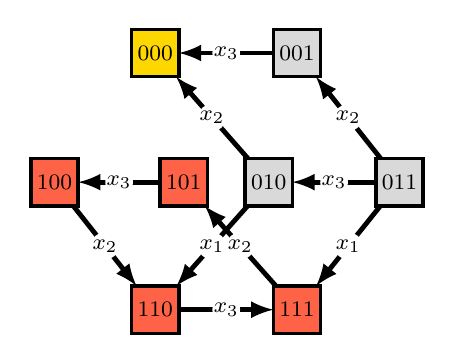
\begin{tikzpicture}[scale=0.8]
				\definecolor{color1}{HTML}{FFD700} %% {rgb}{0.9, 0.756, 0.}
				\definecolor{color2}{gray}{0.85}
				\definecolor{color3}{HTML}{FF6347} %% {rgb}{0.8, 0., 0.}
				\definecolor{color4}{gray}{0.}
				\SetVertexStyle[FillColor=white,MinSize=0.6cm,LineWidth=1.25pt, Shape=rectangle, TextFont=\footnotesize]
				\SetEdgeStyle[TextFont=\footnotesize,LineWidth=1.75] \SetDistanceScale{2.5}
				%% Vertices ------
				\Vertex[x=0.64, y=1.63, color=color1, Math=true, label=000]{0}
				\Vertex[x=1.54, y=1.63, color=color2, Math=true, label=001]{1}
				\Vertex[x=1.36, y=0.81, color=color2, Math=true, label=010]{2}
				\Vertex[x=0.64, y=0, color=color3, Math=true, label=110]{6}
				\Vertex[x=2.19, y=0.81, color=color2, Math=true, label=011]{3}
				\Vertex[x=1.54, y=0, color=color3, Math=true, label=111]{7}
				\Vertex[x=0, y=0.81, color=color3, Math=true, label=100]{4}
				\Vertex[x=0.82, y=0.81, color=color3, Math=true, label=101]{5}
				%% Edges ---------
				\Edge[label=x_1, color=color4, bend=0, Direct=true, Math=true](2)(6)
				\Edge[label=x_3, color=color4, bend=0, Direct=true, Math=true](3)(2)
				\Edge[label=x_1, color=color4, bend=0, Direct=true, Math=true](3)(7)
				\Edge[label=x_3, color=color4, bend=0, Direct=true, Math=true](6)(7)
				\Edge[label=x_2, color=color4, bend=0, Direct=true, Math=true](4)(6)
				\Edge[label=x_3, color=color4, bend=0, Direct=true, Math=true](5)(4)
				\Edge[label=x_2, color=color4, bend=0, Direct=true, Math=true](7)(5)
				\Edge[label=x_2, color=color4, bend=0, Direct=true, Math=true](3)(1)
				\Edge[label=x_3, color=color4, bend=0, Direct=true, Math=true](1)(0)
				\Edge[label=x_2, color=color4, bend=0, Direct=true, Math=true](2)(0)
			\end{tikzpicture}\\
			\textsc{interaction graph}
			\\
			%% INTERACTION GRAPH
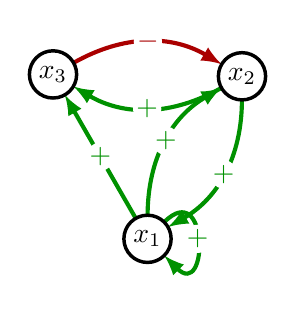
\begin{tikzpicture}[scale=0.8]
	\definecolor{color1}{gray}{1.}
	\definecolor{color2}{rgb}{0., 0.57, 0.}
	\definecolor{color3}{rgb}{0.666667, 0., 0.}
	\SetVertexStyle[FillColor=white,MinSize=0.6cm,LineWidth=1.25pt, Shape=circle, TextFont=\normalsize]
	\SetEdgeStyle[TextFont=\normalsize,LineWidth=1.5] \SetDistanceScale{3.}
	%% Vertices ------
	\Vertex[x=0.50, y=0, color=color1, Math=true, label=x_1]{x1}
	\Vertex[x=1.00, y=0.86, color=color1, Math=true, label=x_2]{x2}
	\Vertex[x=0, y=0.87, color=color1, Math=true, label=x_3]{x3}
	%% Edges ---------
	\Edge[label=+, color=color2, bend=30, Direct=true, Math=true](x1)(x1)
	\Edge[label=+, color=color2, bend=30, Direct=true, Math=true](x1)(x2)
	\Edge[label=+, color=color2, bend=0, Direct=true, Math=true](x1)(x3)
	\Edge[label=+, color=color2, bend=30, Direct=true, Math=true](x2)(x1)
	\Edge[label=+, color=color2, bend=30, Direct=true, Math=true](x2)(x3)
	\Edge[label=-, color=color3, bend=30, Direct=true, Math=true](x3)(x2)
\end{tikzpicture}
		\end{tabu}
		\caption{Asynchronous dynamics and equilibria (in different colors for each attractor), interaction graph}
		\label{fig:boon1}
	\end{figure}

\subsection{Controllability}
	\label{subsec:controllability}
	Recently, a significant body of research
	%% \citep{cifuentes-fontanals2022,pardo2021,biane2019,mandon2019,murrugarra2016,zanudo2015,lin2012,layek2011}
	  has been devoted to the study of controllability in Boolean networks.
The aim of this research is to identify the necessary modifications to the equations governing the network to figure out the means of satisfying a query at a given equilibrium state. The theoretical framework, and the detail of the computational methods developed in \boon for the controllability analysis can be found in\citep{biane2019} and \citep{pardo2021} for its extension to control sequence.

Adding control extends the Boolean network to \emph{Boolean control network} (BCN) where the \emph{control parameters} $u_i$ are added to the equation for figuring the control action.
The classical modifications of equations consist in freezing a variable by setting it to True/$1$ or False/$0$.
Basically, adding control extends the formula to include the control parameters.
A freeze occurs when the control parameters freeze ($u_i=0$) otherwise it is inactive ($u_i=1$). The formalization of the control extension can be achieved as follows for each equation:
\begin{align*}
	x_i &= f_i(x_1, \ldots, x_n) \land u^0_i &\text{for freezing to $0$}\\
	x_i &= f_i(x_1, \ldots, x_n) \lor \neg u^1_i &\text{for freezing to $1$}.
\end{align*}
Note that when $u^0_i = 0$ then the equation becomes $x_i=0$ and similarly when $u^1_i=0$,  $x_i=1$.

The Boolean network~\eqref{eq:boon}, subjected to control thus becomes:
\begin{equation}
	\left\{
	\begin{aligned}
		x_1 &=\left(x_1 \lor x_2\right) \land u^0_1 \lor \neg u^1_1 \\
		x_2 &=\left(\neg x_3\land x_1\right) \land u^0_2 \lor \neg u^1_2 \\
		x_3 &=\left(x_2\land x_1\right) \land u^0_3 \lor \neg u^1_3
	\end{aligned}\right.
	\label{eq:boonctrl}
\end{equation}
The BCN has now $6$ control parameters.

With this method, the control is applied on nodes because the variable is set to a Boolean value when the control freezes.
The control can be also more selectively applied on links\citep{biane2019}.
As the Boolean network is modified when the control freezes, the dynamics is altered leading to different equilibria.

The resolution of control seeks to identify the active control required to fulfill a specified query. This query articulates a condition related to stable equilibria, which may take the following forms:\emph{ possibility}, signifying the existence of at least one stable state that satisfies the query, or \emph{necessity}, mandating that all stable equilibria must conform to the query. The two forms of queries are included in \boon's controllability analysis. 


To illustrate this situation, if the aim is to reach $x_3=1$ at a stable state, the sole control that will achieve this outcome is to activate $u_2^1$ \ie $u_2^1=0$ while $u_i^c=1$ for the other configurations, the resulting BCN and its dynamics are shown in Figure~\ref{fig:bcn}.
Now only one new stable state exists ($111$).
\begin{figure}[h]
	\centering
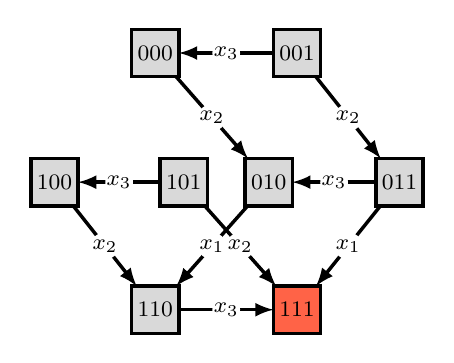
\begin{tikzpicture}[scale=0.8]
	\definecolor{color1}{gray}{0.85}
	\definecolor{color2}{HTML}{FF6347}  %%{rgb}{0.79, 0.16, 0.}
	\definecolor{color3}{gray}{0.}
	\SetVertexStyle[FillColor=white,MinSize=0.6cm,LineWidth=1.25pt, Shape=rectangle, TextFont=\footnotesize]
	\SetEdgeStyle[TextFont=\footnotesize,LineWidth=1.25] \SetDistanceScale{2.5}
	%% Vertices ------
	\Vertex[x=0.64, y=1.63, color=color1, Math=true, label=000]{0}
	\Vertex[x=1.36, y=0.81, color=color1, Math=true, label=010]{2}
	\Vertex[x=1.54, y=1.63, color=color1, Math=true, label=001]{1}
	\Vertex[x=2.19, y=0.81, color=color1, Math=true, label=011]{3}
	\Vertex[x=0.64, y=0, color=color1, Math=true, label=110]{6}
	\Vertex[x=1.54, y=0, color=color2, Math=true, label=111]{7}
	\Vertex[x=0, y=0.81, color=color1, Math=true, label=100]{4}
	\Vertex[x=0.82, y=0.81, color=color1, Math=true, label=101]{5}
	%% Edges ---------
	\Edge[label=x_1, color=color3, bend=0, Direct=true, Math=true](2)(6)
	\Edge[label=x_3, color=color3, bend=0, Direct=true, Math=true](3)(2)
	\Edge[label=x_1, color=color3, bend=0, Direct=true, Math=true](3)(7)
	\Edge[label=x_3, color=color3, bend=0, Direct=true, Math=true](6)(7)
	\Edge[label=x_2, color=color3, bend=0, Direct=true, Math=true](4)(6)
	\Edge[label=x_3, color=color3, bend=0, Direct=true, Math=true](5)(4)
	\Edge[label=x_2, color=color3, bend=0, Direct=true, Math=true](5)(7)
	\Edge[label=x_2, color=color3, bend=0, Direct=true, Math=true](1)(3)
	\Edge[label=x_2, color=color3, bend=0, Direct=true, Math=true](0)(2)
	\Edge[label=x_3, color=color3, bend=0, Direct=true, Math=true](1)(0)
\end{tikzpicture}

$F_{(u_2^1=0)}=\left\{x_1=\left(x_1\lor x_2\right),x_2=1,x_3=\left(x_2\land x_1\right)\right\}.$
\caption{Controlled network of $F$ by assigning $u_2^1=0$.}
\label{fig:bcn}
\end{figure}

The primary challenge is to accurately determine the control parameters' freeze actions to regulate the dynamics to achieve the desired equilibrium.
As previously referenced, a variety of methods have been developed to address this issue.

Controllability analysis is a valuable investigative tool in drug target discovery and disease etiology.
Typically, a biomarker profile identifies a specific state, either disease or healthy.
From control analysis, we can determine which variables should be turned \textsc{on} or \textsc{off}, that is frozen,  in order to achieve the desired binary biomarker profile at stable state.
	This allows us to properly identify the actions that should be applied to genes, either over-expression or inhibition. 
	In the distribution (see \href{https://github.com/Franck-Delaplace/BooN}{GitHub} site), we have fully described an example by a Jupyter program illustrating the use of controllability analysis for the identification of the causes of diseases and the  therapeutic target discovery applied to breast cancer. This analysis is also described in the \textsc{readme} for its interactive application.  

\section{\boon}
	\label{sec:boon}
	\boon facilitates the analysis of the Boolean network including the network design, the equilibrium computation and the controllability analysis.

	\boon has also been added in Colomoto\citep{naldi2018} repository collecting software related to Biological network analysis.
	 The distribution includes the sources, complete documentation of the different methods applied to \boon object, tutorials and various examples including a real application of the controllability analysis on Breast cancer leading to drug target prediction. 
	  \boon is developed in Python and composed of $3$ packages:
	\begin{itemize}
		\item \texttt{boon} is the core library providing a comprehensive set of methods for manipulating the \boon object. 
		\item \texttt{logic} is a sub-library of \texttt{boon} containing the basic functions related to propositional logic, notably: basic functions, formula pretty printing, and prime implicants computation.
		\item \texttt{boonify} is the user-friendly graphical interface (GUI) interfacing the \texttt{boon} function based on  \texttt{PyQT5}.
	\end{itemize}
    \boon has an internal file format for the storage of Boolean networks.
    However, for interoperability with other applications, Boolean networks in BoolNet, SBML, or Python-based format can also be imported.

	Figure~\ref{fig:BooNGUI} illustrates the full range of analysis features accessible via different windows using the GUI for Boolean network~\eqref{eq:boon}.
	
	\begin{figure}[htb]
		\centering
		\begin{tikzpicture}
			\definecolor{wingray}{gray}{0.95}
			\node[inner sep=0pt] (boongui) at (3,2)
			{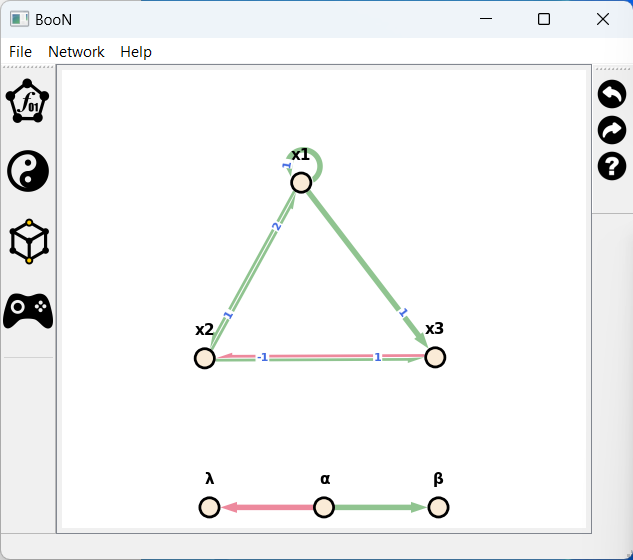
\includegraphics[width=5cm]{boongui.png}};
			\node[inner sep=0pt] (view) at (0,-0.5)
			{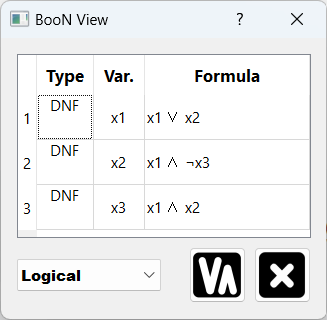
\includegraphics[width=3cm]{view.png}};
			\node[inner sep=0pt] (dynamics) at (5.5,5.2)
			{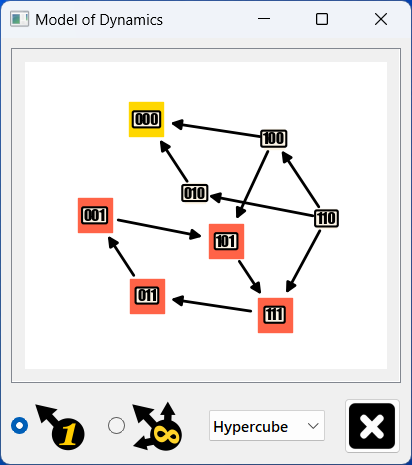
\includegraphics[width=3.5cm]{dynamics.png}};
			\node[inner sep=0pt] (controllability) at (1.,5.5)
			{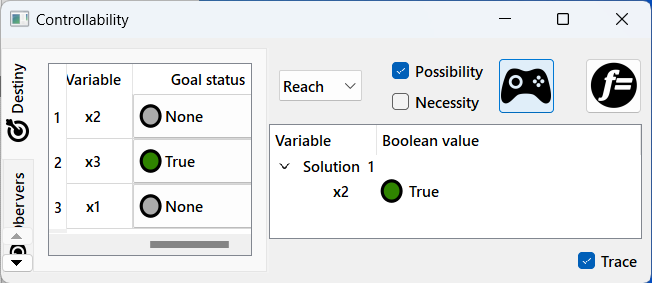
\includegraphics[width=5cm]{controllability.png}};
			\node[inner sep=0pt] (stablestate) at (5.75,0)
			{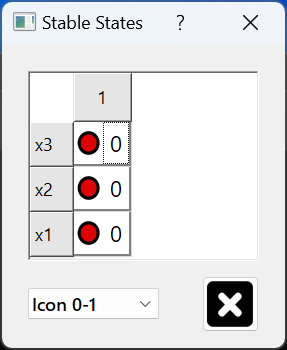
\includegraphics[width=3cm]{stablestate.png}};
			
			\tikzstyle{txt}=[draw,shape=rectangle,fill=wingray,font=\scriptsize, inner sep=1ex]
			\node[txt]  at (2.1,3.4) {Network Design};
			\node[txt]  at (-0.5,1.25) {Formulas View};
			\node[txt]  at (5.75,2.15) {Symbolic Stable States};
			\node[txt]  at (6.3,6.4) {Dynamics};
			\node[txt]  at (0,6.9) {Controllability Analysis};
		\end{tikzpicture}
		\caption{Overview of the \boon functionalities/windows using GUI.}
		\label{fig:BooNGUI}
	\end{figure}
	
	Concerning the GUI, the design of the Boolean network is completely achieved from the drawing of the interaction graph (Figure~\ref{fig:BooNGUI}). From the interaction graph drawing a \textsc{dnf} formula is generated. Therefore there is no conceptual limitation on the formulas since all formulas can be converted to \textsc{dnf}. The user draws the positive or the negative interactions and specifies in which module the variable belongs. A module characterize a set of cooperative variables. It is identified by an integer id and translated into a AND-clause in the \textsc{dnf} formula. Also note that the formula can be modified directly using the Formula View.  
	 
	Moreover, the different analysis (Dynamics w.r.t.\ a mode, Controllability, symbolic Stable state computation) are accessible via a menu and buttons located in the both sides of the main window where the interaction graph is drawn.
	Comprehensive online help is also available. 

	More technically, the dynamics refers to calculating transitions between states in a mode that defines the state updating policy. The full dynamics computation is available in \boon in both the synchronous and asynchronous modes, and more generally for any possible mode.

	The symbolic computation of stable states efficiently lists the interpretations of the following equivalence stating the fixed point of the dynamics:
	 $ f(x) \iff x.$
	 The resolution is achieved by a SAT solver, specifically the Z3-Solver. %% \citep{demoura2008}
	
	Moreover, the controllability analysis entails the computation of prime implicants, as detailed in the reference\citep{biane2019}.
	These prime implicants are used to extract the active control parameters which define the control to be applied. 
	
	Given that a control is active if it is equal to $0$ ($u_i^c=0$), we extract the negative control parameters from the prime implicants, which are true only when they are set to $0$, for the purpose of defining the core, which is the minimal set of active control parameters under the inclusion. The other variables,positive controls and network variables, are discarded since they do not share information related to the control activity. 
	The prime implicant algorithm that has been implemented is based on the translation of the problem into an integer linear programming problem\citep{pizzuti1996} and the integer linear programming solver used is PULP.
	
	\section{Method performance}
	\begin{figure}[h]
		\centering
		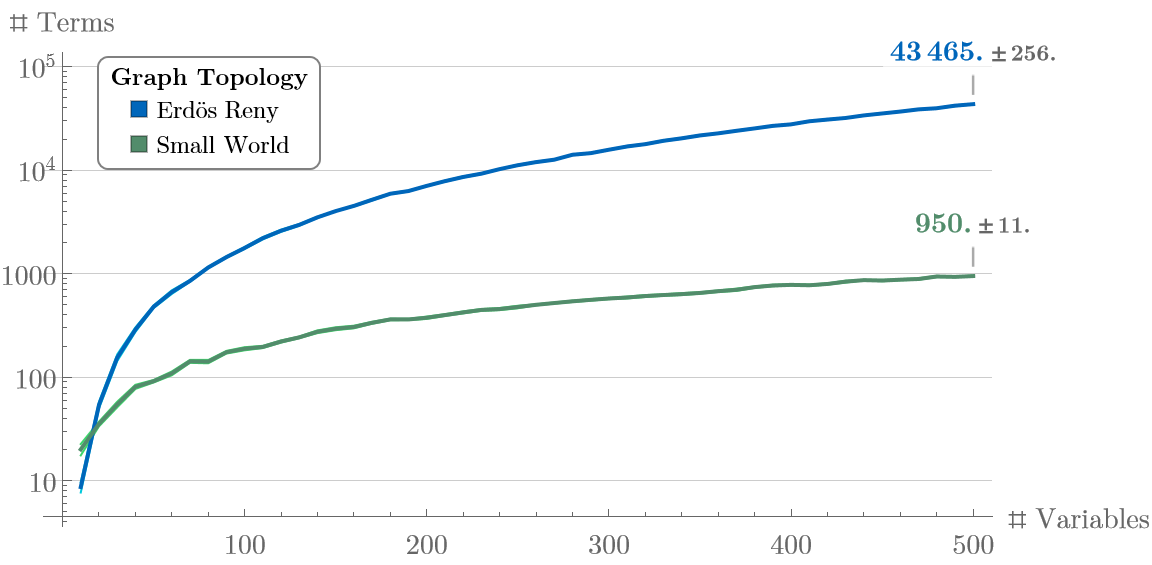
\includegraphics[width=0.45\textwidth]{number-terms}
		
		\caption{Number of terms per network size and topology.}
		\label{fig:terms}	
	\end{figure}
	The primary methods of \boon are benchmarked using randomly generated Boolean networks. We classified these networks into two categories based on the topology of their interaction graphs: Erdős-Rényi and Small-World. The formulas were constructed from interaction graphs defining variable dependencies. For each variable,a \textsc{dnf} formula is randomly generated from the input neighbors of the variable within the interaction graph. The number of clauses is randomly defined within predefined bounds, and the negations are determined from a parameter controlling the likelihood of positive terms. Formulas derived from the Erdős-Rényi interaction graph proved more complex, containing a greater number of terms than those from the Small-World interaction graph (Figure~\ref{fig:terms}). Consequently, the benchmark analysis is divided into two formula categories: complex formulas (Erdős-Rényi) and simpler formulas (Small-World). The benchmark was computed on a \textsc{Intel} Icore 7 (1.90 Ghz) with 16Go of RAM.
	
	 The benchmark assesses the efficiency of the methods on networks of increasing size in terms of the number of variables. For each size, 10 networks are randomly generated. The curves show the average for each size with its uncertainty. The benchmark Jupyter program is included in the GitHub release. We respectively assess the stable state computation, the brute force equilibria computation and the controllability analysis.
	\label{sec:benchmark}

	 
\subsection{Stable states}
			\begin{figure}[h]
		\centering
		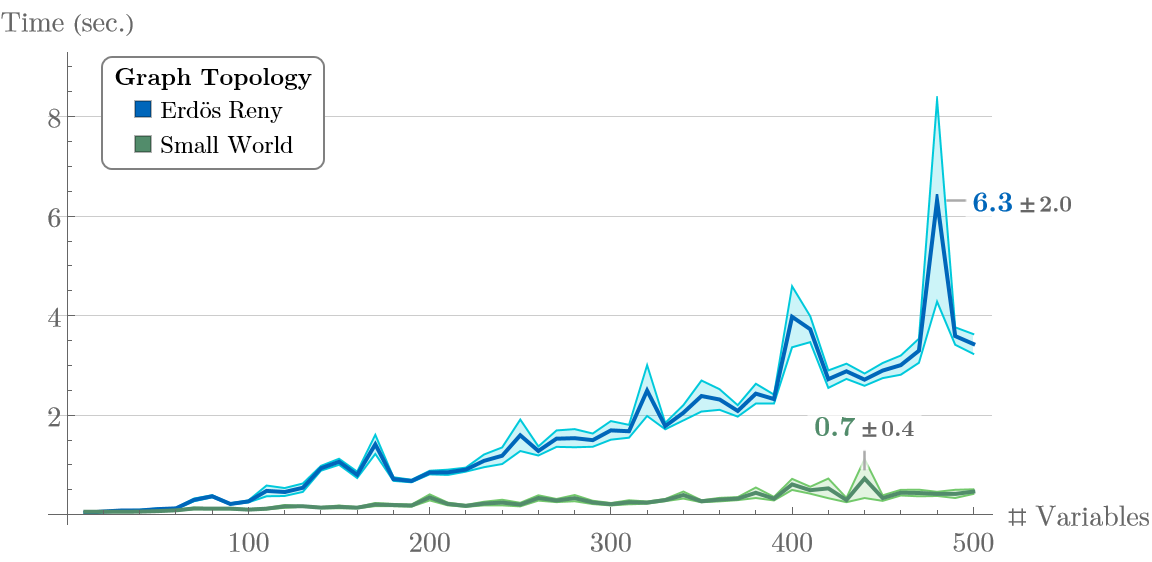
\includegraphics[width=0.45\textwidth]{stable-state-bench}
		
		\caption{Time for stable states computation.}
		\label{fig:stable state}	
	\end{figure}
	The stable state method based on symbolic resolution using the Z3-solver is a very fast and scalable approach, with processing times of less than $6.3~sec$ for large networks comprising thousands of terms~(Figure~\ref{fig:terms}). The complexity of the formulas has a significant impact of the time computation.  

\subsection{Equilibria}
		\begin{figure}[!h]
	\centering
	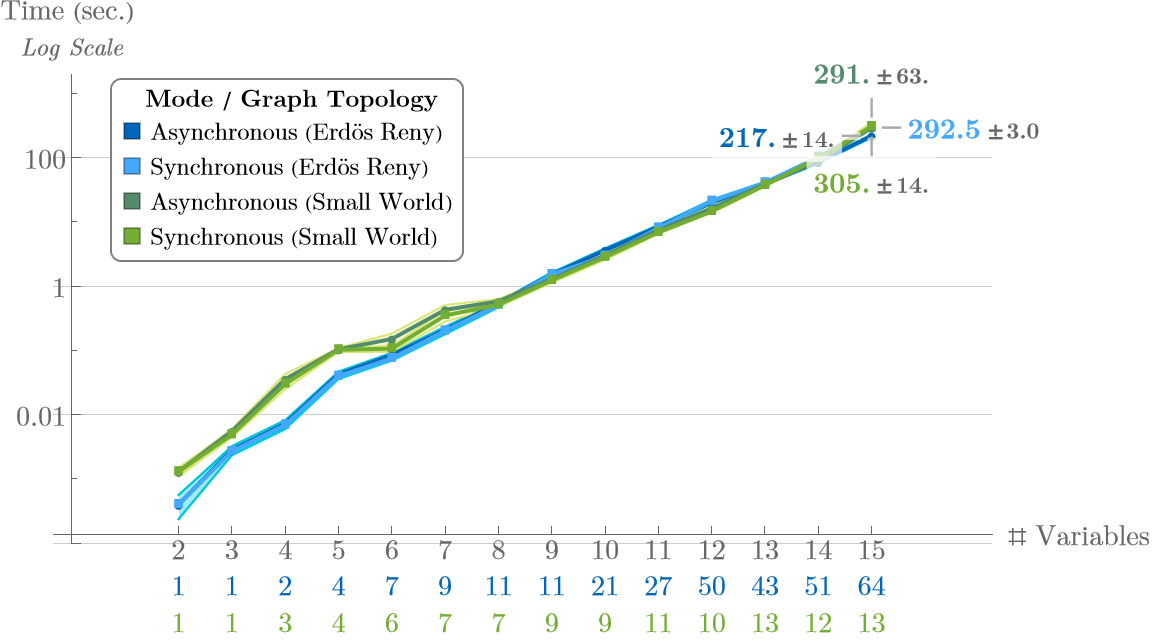
\includegraphics[width=0.45\textwidth]{equilibria-bench}
	\begin{tablenotes}
		Below the number of variables is the number of terms for the Erdos-Reny and Small-World networks.
	\end{tablenotes}
	
	\caption{Time for equilibria computation.}
	\label{fig:stable state}	
\end{figure} 

	The brute force algorithm characterizing the attractors is performed on the whole state space ($2^{|X|}$ states).  As might be expected, the time required is doubled with each additional variable, and thus follows an exponential growth curve. Nevertheless, the algorithm has been optimized to remain efficient when considering a limited number of variables, which in this case is $15$. Our analysis revealed no notable discrepancies between the Small-World and Erdös-Reny formulas. This is because the primary constraint stems from the exponential number of states, rather than the complexity of the formulas themselves.


\subsection{Controllability}
	The final benchmark pertains to the evaluation of controllability.  The queries ascertain some requisite conditions corresponding to a Boolean profile for the variables $x_0$ and $x_1$. 
	 The selected profile is never satisfied in the current stable states. The goal is to possibly reach this profile at stable state (in $1$ stable state at least). 

	 This benchmark demonstrates that the controllability method is efficient for the typical Boolean networks designed to model genetic networks, the majority of which have around $30$ nodes and rarely exceed $50$. However, the performance is contingent on the complexity of the formulas, thereby explaining the observed time difference between Erdös-Renyi and small-world networks. Indeed, the number of terms has a direct influence on the resolution capability of the PULP ILP-solver, since the system to be solved will be more complex. 
	 	\begin{figure}[h]
	 	\centering
	 	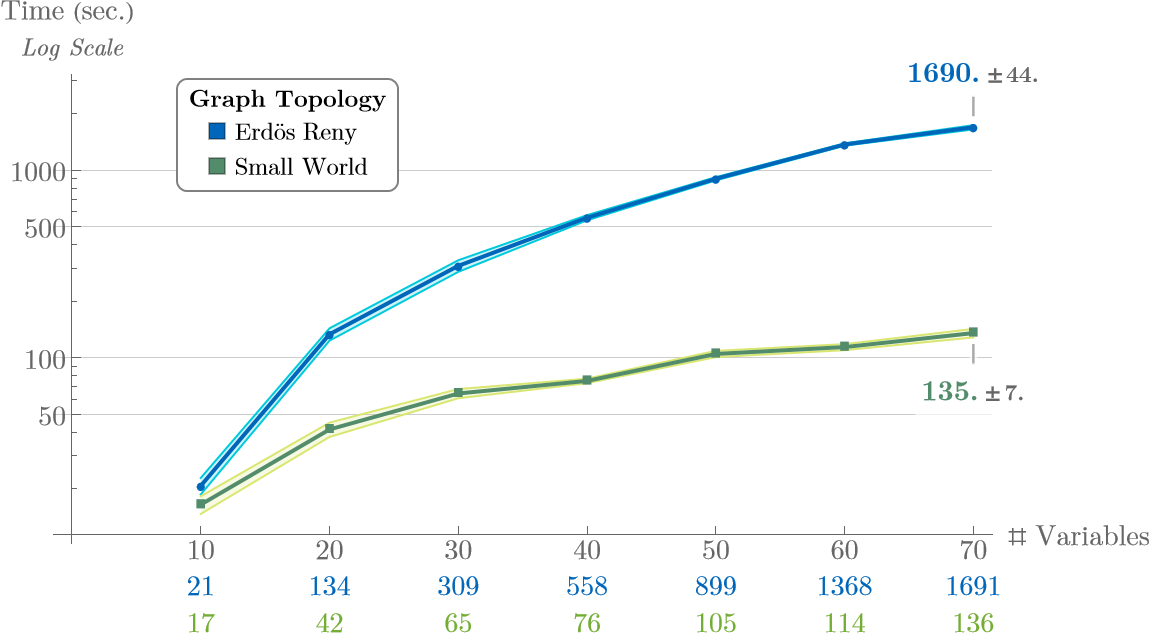
\includegraphics[width=0.45\textwidth]{possibility-bench}
	 	\begin{tablenotes}
	 		Below the number of variables is the number of terms for the Erdös-Reny and Small-World networks.
	 	\end{tablenotes}
	 	
	 	
	 	\caption{Time evaluation for controllability (possibility) queries.}
	 	\label{fig:stable state}	
	 \end{figure}

	
	\section{Conclusion}
	\label{sec:conclusion}
	
 	 \boon provides a python package for Boolean network analysis and a graphical interface which provides a convenient way to visualize and interact with the network. It also offers unique capabilities for controllability analysis, which is not available in other software.
 
 	A number of software applications are devoted to controllability analysis, as \textsc{cabean}~\citep{su2021} or Bonesis\citep{chevalier2024}.
 	However, they are focused on this specific analysis and do not encompass the other aspects related to Boolean dynamics analysis.
 
 	In conclusion, \boon is a software solution tailored for Boolean network dynamics analysis, featuring a unique ability to conduct controllability analysis.
 	Furthermore, its  graphical interface allows for the straightforward manipulation of Boolean networks.

%% \bibliographystyle{abbrvnat}
%% \bibliographystyle{bioinformatics}
\bibliographystyle{apalike}
\bibliography{BibBooN}
\end{document}